\documentclass{IEEEtran}
\usepackage{graphicx}
\usepackage{hyperref}
\usepackage{amsmath}
\usepackage{cite}
\usepackage{booktabs}
\usepackage{caption}
\usepackage{amsfonts}
\usepackage{listings}
\usepackage{array}
\usepackage{mathtools}
\newcolumntype{P}[1]{>{\centering\arraybackslash}p{#1}}
\DeclareCaptionType{equ}[][]

\DeclarePairedDelimiter\abs{\lvert}{\rvert}%
\DeclarePairedDelimiter\norm{\lVert}{\rVert}%

\makeatletter
\let\oldabs\abs
\def\abs{\@ifstar{\oldabs}{\oldabs*}}

\let\oldnorm\norm
\def\norm{\@ifstar{\oldnorm}{\oldnorm*}}
\makeatother

\markboth{Kernels methods for machine learning : Class 2022-2023, MVA MSc}{Last Name \MakeLowercase{\textit{et al.}}: Title}

\title{
    \huge{
        Report on the Kaggle Data Project
        for
        MVA 22-23 Kernels Methods Class.
        }
}
\author{Louis BLAZEJCZAK-BOULEGUE, Romain SÉAILLES\\
Kernels Methods for Machine Learning Class 2022-2023, MVA MSc\\
    \{louis.blazejczak-boulegue, romain.seailles\}@etu.minesparis.psl.eu
}
\begin{document}
\maketitle

\section{The Challenge}

The goal of this challenge was to process molecules represented as graphs and predict their activity based on their structure. The key requirement for the challenge was to accomplish this task using kernel methods only. This challenge took place in our MVA class, and it presented an opportunity to learn how to implement machine learning algorithms using kernel methods.

The available data were a training dataset composed of 6000 annotated molecules used for training and 1000 non-annotated molecules for testing purposes. Teams were required to submit their predictions for the test set to Kaggle for evaluation.

\section{Pipeline}

\subsection{Structure}
We choose to develop using Python and C++ mainly.

Our project's structure looks like this:

\begin{figure}[h]
    \begin{lstlisting}[frame=none,basicstyle=\ttfamily]
        project/
        |-- data/
        |-- export/
        |-- kernels/
        |-- rapport/
        |-- results/
        |-- biblio/
        |-- dataset/
        |-- optimization/
        |-- run.py
        |-- treeEditDistance/
        |-- configs/
        |-- env/
        |-- preprocessing/
        |-- requirements.txt
        `-- svc/
    \end{lstlisting}
    \captionof{figure}{Project Structure}
    \label{fig:project-structure}
\end{figure}


Here is a brief presentation of the contents:

\begin{itemize}
    \item \texttt{data/}: This folder contains test and training datasets and labels.
    \item \texttt{export/}: This folder contains the resulting \texttt{.csv} file after running kernels that can be submitted to Kaggle.
    \item \texttt{kernels/}: This is where all the kernel code is located. It contains the main class kernel, as well as every subclass implementing a different kernel.
    \item \texttt{rapport/}: This folder contains the Latex files used to produce this article.
    \item \texttt{results/}: This folder contains all the results tables for each run, used for comparison purposes.
    \item \texttt{biblio/}: This folder contains biobliographic references we read.
    \item \texttt{dataset/}: This folder includes our custom dataset class. It is designed around our cross-validation mecanic. This will be detailed later on.
    \item \texttt{optimization/}: This folder contains the framework to tune the hyperparameters of our kernel using a Bayesian search algorithm.
    \item \texttt{run.py}: This is the main entry point of our program. It can evaluate the performance of a given kernel and produce predictions on the test dataset.
    \item \texttt{treeEditDistance/}: This is a Python module written in C++ useful to compute the Generalized Wasserstein Weisfeiler-Lehman kernel, which will be detailed later on.
    \item \texttt{configs/}: This folder contains all the configured kernels. A unique kernel can be deployed using multiple config files with different parameters. For instance, there is only one Weisfeiler-Lehman kernel class, but there are multiple Weisfeiler-Lehman config files that deploy this kernel with different depths. Those config files are given to \texttt{run.py} to be evaluated and tested.
    \item \texttt{env/}: This folder contains our Python environment.
    \item \texttt{preprocessing/}: This folder includes useful functions such as \texttt{load\_data}, for example.
    \item \texttt{requirements.txt}: This file lists all our Python dependencies.
    \item \texttt{svc/}: This folder implements our custom Support Vector Classifier (SVC) implementation.
\end{itemize}

Note that we deployed several \texttt{unittest}s to test important objects, especially SVC and kernels. These were tested against the well-known \texttt{scikit-learn} implementation. This protocol ensures that any modification, especially towards optimization, will not break our work pipeline. Furthermore, it ensures that our tools are accurate and that our results are reproducible.

\subsection{Comparing different solutions}
We performed cross-validation to compare the effectiveness of different kernels. We chose to use a 6-fold cross-validation process on the molecule dataset, which consisted of 6000 molecules. The dataset was randomly split into six sets of 1000 molecules each, with a fixed seed for reproducibility.

For each fold in the cross-validation process, one set was separated for testing while the other five were used for training. This means that each fold involved training a Support Vector Classifier (SVC) on 83\% of the data and testing it on the remaining 17\%.

Given the heaviness of the class imbalance in our dataset,
we opted to track the F1 score metric. We also measured accuracy, precision, and recall for informational purposes.
However, we mainly relied on the ROCAUC to evaluate the performance of our project, as it was the metric chosen to rank the leaderboard on Kaggle.

Table \ref{tab:example} shows the results of our tests for one kernel.
Similar output tables for all tested kernels are store in the \texttt{results/} directory,
and all our results are available in the Appendix \ref{appendix:allresults}.

\begin{table}[h]
    \centering
    \begin{tabular}{l||llll|l}
                & Accuracy & Precision & Recall & F1     & ROCAUC \\
        \hline \hline
        Fold 1  & 93.0\%   & 52.2\%    & 64.9\% & 57.8\% & 88.2\% \\
        Fold 2  & 88.3\%   & 47.3\%    & 74.1\% & 57.8\% & 89.4\% \\
        Fold 3  & 88.2\%   & 40.0\%    & 77.6\% & 52.8\% & 89.5\% \\
        Fold 4  & 92.1\%   & 65.9\%    & 54.2\% & 59.5\% & 88.0\% \\
        Fold 5  & 93.1\%   & 64.0\%    & 53.3\% & 58.2\% & 87.9\% \\
        Fold 6  & 93.0\%   & 61.3\%    & 62.6\% & 62.0\% & 90.8\% \\
        \hline
        Average & 91.3\%   & 55.1\%    & 64.5\% & 58.0\% & 89.0\% \\
    \end{tabular}
    \caption{Example of the output table for one of the tested kernels, \emph{WL-depth4} \ref{tab:wwl}.}
    \label{tab:example}
\end{table}


\subsection{Optimizing a solution}
To optimize our kernel parameters, we used the same 6-fold cross-validation method as previously mentioned. However, in this step, we performed a Bayesian search within a parameter grid to obtain optimal values.

This method is highly efficient in fine-tuning parameters because it can optimize functions that are computationally expensive and where gradient computation is not possible \cite{stone1976theory}.
All the results that we present in this report correspond to the best version of a kernel obtained after hyperparameter tuning.

\subsection{Faster Inference}
As we will soon discuss, computing kernels with graphs can be quite expensive. Therefore, it was mandatory to optimize our code as much as possible to avoid any loss of time and ensure optimal overall performance.

Firstly, the kernel's Gram matrix was pre-computed when possible and then split according to specific indices for each fold. This strategy prevents expensive recomputations. Otherwise, it is calculated on the fly when fitting the SVC and only half of the matrix has to be computed as the matrix is symmetric.

Furthermore, nearly all our kernels can be decomposed into two steps of different complexity:
a heavy step computing an embedding of a graph (similar to the embedding $\phi(x)$ in the RKHS)
and a lighter operation between those two embeddings (similar to the inner product in the RKHS).
Given the pipeline before, with one subset of graphs (resp. two) of size
$n$ (resp. $n,m$), one can see that the heavy method $\phi$ can only be called
$n$ (resp $n+m$) times at the beginning,
while the lighter operation will be called to fill the Gram matrix
- only its upper-triangular part in the one-subset case -
which leads to $n(n+1)/2$ operations (resp $n*m$).
Separating these operations drastically increases performance
as it decreases the program's complexity
by one degree.

Finally, we deployed multiprocessing to use as many cores as possible and make the calculation as fast as possible. Special attention was given to using only NumPy's methods as they are compiled in C and thus faster than Python's inherent operations.

Some kernels (especially the Generalized Wasserstein Weisfeiler-Lehman) were still too slow even with these tricks, so we decided to recreate them in C++, which is significantly faster than Python due to its compiled nature. Furthermore, we also moved the outer loop (computing the gram matrix) in the C++ module to benefit from native multithreading and avoid any useless back and forth between Python and our module. Finally, we implemented a caching system to avoid re-computing redundant operations when possible.

\subsection{Our code}
Our complete project is published on GitHub and can be accessed at \url{https://github.com/RSLLES/KernelMethodsDataChallenge}.
\section{Support Vector Classifier (SVC)}

The implemented Support Vector Classifier solves the dual of the C-SVC problem with hinge loss:
given $n$ observations $x_i$ and labels $y_i$ and a kernel $K$,
the primal problem is to find a function $f$ in $\mathcal{H}$ the RKHS of $K$ such that

\begin{equation}
    \label{eq:primal_svc}
    \begin{split}
        \min_{f, b, \xi_i} & \frac{1}{2} \norm{f}_\mathcal{H}^2 + C\sum_i \xi_i\\
        \text{s.t.} & y_i\left( f(x_i) + b \right) \geq 1 - \xi_i\\
        & \xi_i \geq 0
    \end{split}
\end{equation}

where $\xi_i$ represents the margin and $b$ some constant offset.
The problem formulates the separation of classes $y = \pm 1$ in $\mathcal{H}$ by the $f(x) + b = 0$ hyperplane in the RKHS by minimizing the hinge loss $\max\left(0, 1 - y_i\left(f(x_i) + b\right)\right)$.
The margin $\xi_i$ is a slack variable that allows the model to do some misclassification because learning a very complex separation boundary in the RKHS leads to overfitting: regularization helps retaining generality.

The dual problem of~\ref{eq:primal_svc} involves the pairwise kernel matrix $\tilde{K}$ :

\begin{equation}
    \label{eq:dual_svc}
    \begin{split}
        \min_{\alpha} & \frac{1}{2} \alpha^T M \alpha - \sum_i \alpha_i\\
        \text{s.t.} & \alpha^T y = 0\\
        & \tilde{C} - \tilde{A}\alpha \geq 0\\
        \text{where} & M = \text{diag}(y) \tilde{K} \text{diag}(y)\\
        & \tilde{C} = \begin{pmatrix} C & \dots & C & 1 & \dots & 1 \end{pmatrix}^T \text{ (vector of size }2n \text{)}\\
        & \tilde{A} = \begin{pmatrix} I_n \\ -I_n \end{pmatrix}
    \end{split}
\end{equation}

where $\alpha$ (vector of size $n$) represents the dual variables.

We solve the dual problem, which is convex (a quadratic program) using the \texttt{cvxpy} package which contains a symbolic interface and solvers for many types of convex problems.
We focused our development efforts towards producing a similar interface to the \texttt{scikit-learn} interface for most classifiers.
Indeed, although we did not use \texttt{scikit-learn} to perform any prediction for the challenge, we used it to validate our implementation of SVC through unit tests: our end-to-end tests require our implementation to output exactly the same results as \texttt{scikit-learn}'s implementation on some toy data.
Once our implementation was validated on simple examples, we could safely perform predictions with graph kernels applied on the challenge's data.
Given the fact that this is significantly more computationally intensive, this testing step was crucial to ensure our resources were well invested.

\section{Kernels}

The literature on graph kernels is vast and constantly
evolving due to active research and development.
To begin our work, we reviewed the literature and explored
state-of-the-art kernel techniques for the current solution.
Considering its recent good performance,
we chose to focus on variants of the Weisfeiler-Lehman Kernel \cite{shervashidze11a}.

\subsection{Weisfeiler-Lehman (WL)}
As part of our project, we implemented and experimented with the Weisfeiler-Lehman (WL) method,
a graph isomorphism algorithm originally designed by Weisfeiler and Lehman in 1968 \cite{weisfeilerlehman1968}.
The algorithm aims to determine if two graphs are isomorphic with one-sided error.

The core idea of the Weisfeiler-Lehman method is to repeatedly refine a partition of the vertex set, where each node's label and those of its neighbors are concatenated, sorted, and hashed to produce a new label. The hash function employed by the algorithm should be as perfect as possible, meaning that different sets of labels should never be mapped to the same new label. With each iteration, larger substructures are incorporated into the labels, allowing the algorithm to capture more complex patterns in the graph. Finally, the new graphs after each iteration can be compared using a relatively simple algorithm, as the deeper the algorithm goes, the more information is encapsulated from the neighborhood of every node inside its label.

Figure~\ref{fig:wlmethod} - extracted from~\cite{shervashidze11a} - details the process.

\begin{figure}[h]
    \centering
    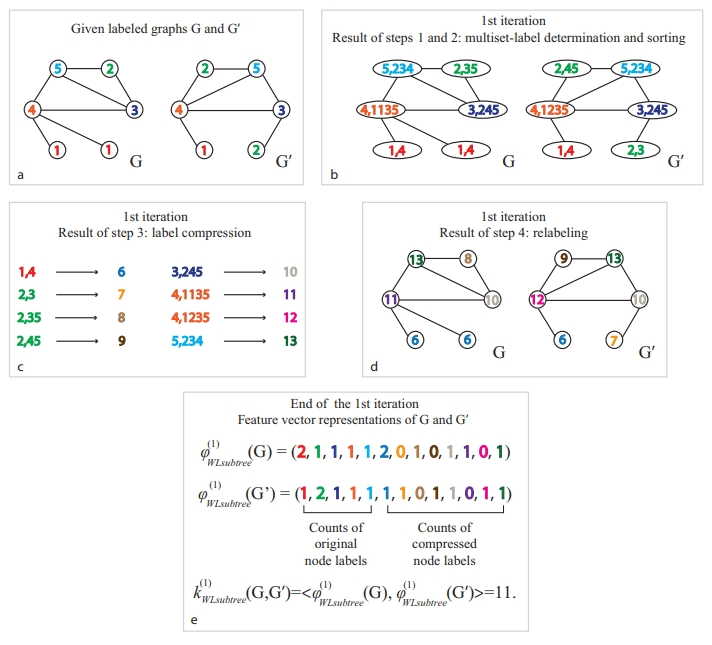
\includegraphics[width=\linewidth]{wl_process.jpg}
    \caption{The Weisfeiler-Lehman Method.}
    \label{fig:wlmethod}
\end{figure}

Moreover, this kernel is exceptionally computationally efficient.
Indeed, all the embeddings can be computed separately for each node,
and the final comparison is quite simple,
resulting in an overall high efficiency.

A fast and straightforward approach to compare graphs would be to evaluate the frequency of their nodes.
For each subgraph iteratively computed during the Weisfeiler-Lehman process,
all of its nodes can be compared with all the nodes of another graph,
using a Kronecker metric.
More formally, given two graphs $G_1$ and $G_2$
with respective set of nodes $\mathcal{N}_1$, $\mathcal{N}_2$, let $l(n)$
be the label associated with the node $n$ in either $\mathcal{N}_1$ or $\mathcal{N}_2$.
Then the proposed kernel can be formulated as:

\begin{equation*}
    K(G_1, G_2) = \sum_{n_1 \in \mathcal{N}_1} \sum_{n_2 \in \mathcal{N}_2} [1 - \delta_{l(n_1), l(n_2)}]
\end{equation*}
where $\delta_{l(n_1), l(n_2)} = 1$ \text{ if } $l(n_1) = l(n_2)$ and $0$ otherwise.

This approach is known as the Weisfeiler-Lehman Subtree Kernel, and it has been widely studied in the literature.
We prove that this kernel is positive semi-definite.
First, note that every label is an integer,
as we use a hash function from $\mathbb N $ to $\mathbb N $.
We embed a node $n$ with a sequence $u^{(n)}$ such that
$\forall k \in \mathbb{N}, u^{(n)}k = 1$ if $k = l(n)$, 0 otherwise.
As each node has a unique label, $\sum{k=0}^\infty u^{(n)}_k = 1$,
hence it is absolutely convergent, and thus, the following scalar product is well-defined over the space of absolute convergent sequences:

\begin{equation*}
    \forall u^{(n_1)}, u^{(n_2)}, < u^{(n_1)} \; | \; u^{(n_2)} > =
    \sum_{k=0}^\infty u^{(n_2)}_k u^{(n_1)}_k
\end{equation*}

Therefore, the kernel is positive definite.

Given a sequence of graphs $G^{(k)}$ obtained after the $k$-iteration of the Weisfeiler-Lehman process,
one can simply sum the results of the kernel described above at each level, creating a positive definite kernel.

After optimization, we found that this kernel achieves its best performances using a depth of $5$.
Results are presented in Table \ref{tab:wldepth5}.

\begin{table}[h]
    \centering
    \begin{tabular}{l|llll|l}
                & Accuracy & Precision & Recall & F1     & ROCAUC \\
        \hline
        Average & 92.6\%   & 61.1\%    & 58\%   & 59.1\% & 89.3\% \\
    \end{tabular}
    \caption{\emph{WL-depth5} performances.}
    \label{tab:wldepth5}
\end{table}

The code for this kernel is available in our repository : \texttt{kernel/WL.py}.

\subsection{Weisfeiler-Lehman-edges}
The previous model did not take into account the labels associated with edges. To address this issue, we chose to include the label of the edge in the label of a node's neighborhood when constructing its new label in the Weisfeiler-Lehman scheme.

Previously, given a node $n$ in a graph $G$, when considering one of its neighbors $n'$, we used $l(n')$ as the label for $n'$. However, we now consider $\operatorname*{hash}(l(n'), l(\operatorname{edge}(n, n')))$,
which combines the labels of the neighbor node ($n'$) with the label of the edge that connects it to the considered node ($\operatorname{edge}(n, n')$).

We found that this simple modification led to a significant improvement in retrieval performance.
As shown in Table~\ref{tab:wldepth6edge}, the average accuracy, precision, F1-score, and ROCAUC increased when we applied this modification.


\begin{table}[h]
    \centering
    \begin{tabular}{l|llll|l}
                & Accuracy & Precision & Recall & F1     & ROCAUC \\
        \hline
        Average & 93.0\%   & 64.0\%    & 55.1\% & 59.2\% & 90.3\% \\
    \end{tabular}
    \caption{\emph{WL-edge-depth6} performances.}
    \label{tab:wldepth6edge}
\end{table}

From our experiments with various kernels, we observed that adding the edge label information in the Weisfeiler-Lehman process consistently led to better performance. Therefore, all of the following kernels include this modification, even if it is not specified explicitly.

The code for this kernel is available in our repository : \texttt{kernel/WL.py}
with \texttt{edges\_labels = True}.

\subsection{Weisfeiler-Lehman variants}
Since the Weisfeiler-Lehman Subtree Kernel is based on a relatively simple update scheme,
we believe that there is room for improvements in this area.

To begin with, we note that the previous version of the Weisfeiler-Lehman Subtree Kernel can be reformulated
as a Vertex Histogram Kernel. Indeed,
given a graph $G$, we denote by $m_G(l(n))$ the multiplicity of
the label $l(n)$ in the graph $G$ (with $m_G(l(n)) = 0$ if $n$ is not an
element of $\mathcal N_G$). Denoting by $L_G = \{l(n), n \in \mathcal N_G\}$
the set containing all the labels of the nodes in $G$,
one can easily check that these two formulations are equivalent:
\begin{equation*}
    \begin{split}
        K(G_1, G_2) & = \sum_{n_1 \in \mathcal{N}_1} \sum_{n_2 \in \mathcal{N}_2} [1 - \delta_{l(n_1), l(n_2)}]\\
        &= \sum_{l \in L_{G_1} \cup L_{G_2}} m_{G_1}(l)m_{G_2}(l)
    \end{split}
\end{equation*}

Therefore, we tried slightly varying this kernel, based on the kernel presented in class as an exercise:

\begin{itemize}
    \item The Minimum Vertex Histogram Kernel (min-WL)

          \begin{equation*}
              K(G_1, G_2) = \sum_{l \in L_{G_1} \cup L_{G_2}} \operatorname*{min}(m_{G_1}(l), m_{G_2}(l))
          \end{equation*}

    \item The Min over Max Vertex Histogram Kernel (minmax-WL)
          \begin{equation*}
              K(G_1, G_2) = \sum_{l \in L_{G_1} \cup L_{G_2}} \frac{\operatorname*{min}(m_{G_1}(l), m_{G_2}(l))}{\operatorname*{max}(m_{G_1}(l), m_{G_2}(l))}
          \end{equation*}
    \item The Arithmetic Vertex Histogram Kernel (arithm-WL)
          \begin{equation*}
              K(G_1, G_2) = \sum_{l \in L_{G_1} \cup L_{G_2}} \frac{\operatorname*{GCD}(m_{G_1}(l), m_{G_2}(l))}{\operatorname*{LCM}(m_{G_1}(l), m_{G_2}(l))}
          \end{equation*}
\end{itemize}

Overall, these slight variants performed below our last baseline \emph{WL-edges-depth6}.
Results can be found in Table~\ref{tab:method_comparison_depth4}.
\begin{table}[h]
    \centering
    \begin{tabular}{l|llll|l}
        Method    & Accuracy & Precision & Recall & F1     & ROCAUC \\
        \hline
        min-WL    & 93.2\%   & 64.9\%    & 57.8\% & 61\%   & 89.7\% \\
        minmax-WL & 93.3\%   & 67.1\%    & 54\%   & 59.8\% & 89.3\% \\
        arithm-WL & 93.4\%   & 67.7\%    & 54.3\% & 60.3\% & 88.5\% \\
    \end{tabular}
    \caption{Performances of Min-WL, MinMax-WL and Arithm-WL at depth 4 with edges.}
    \label{tab:method_comparison_depth4}
\end{table}

The code for those kernels is available in our repository : \texttt{kernel/WL.py}.

\subsection{Jensen-Shannon Weisfeiler-Lehman Kernel (JSWL)}

During our search for new kernels to try, we realized that the Vertex Histogram Kernel formulations (which refer to the frequency of each label inside a given graph) could be interpreted as a probability measure after normalization.
Formally, given a graph $G$, we could extract a probabilty measure
$\rho$ such that :

\begin{equation*}
    \forall l \in \mathbb N, \rho (l) = \frac{m_G(l)}{\sum_{\lambda \in L_G}{m_G(\lambda)}}
\end{equation*}

We were now facing the question of comparing two probability measures.
The first idea that came into our mind was to use Kullback-Leibler divergence.
Unfortunately, this divergence is not symmetric and therefore cannot be used as a kernel.
However during our research, we found the Jensen-Shannon divergence,
that is a smooth and symmetric version of the Kullback-Leibler divergence ~\cite{callut2011sequence}.

Given two probabilty distribution $P$ and $Q$, we denote their
Jensen-Shannon divergence as :

\begin{equation*}
    JS(P, Q) = \frac{1}{2}KL(P|M) + \frac{1}{2}KL(Q|M)
\end{equation*}
where $M = \frac{1}{2} \left( Q + P \right)$ and $KL$ is the Kullback-Leibler divergence.

After some additionnal searching, we found that the Jensen-Shannon divergence is a conditional negative function \cite{callut2011sequence}.
Therefore, according to a theorem we found in~\cite{callut2011sequence},
given a conditional negative function $ f : \mathcal{X} \times \mathcal{X} \to R$,
the kernel $K : \mathcal{X} \times \mathcal{X} \to R$ defined such that:
$\forall x, y \in \mathcal{X}, K(x, y) = \exp{(- \lambda f(x,y))}$
is positive definite with $\lambda > 0$.

Furthermore, a nice property of this kernel is
that the Jensen-Shannon divergence can be rewritten using the
the Shannon entropy, denoted $H$. It can be shown that:

\begin{equation*}
    JS(P, Q) = H(M) - \frac{1}{2} \left( H(Q) + H(P) \right)
\end{equation*}
The attentive reader might notice that
$H(P)$ and $H(Q)$ can be precomputed ahead of time,
leading to a very fast implementation.

The results using this kernel are shown in Table~\ref{tab:jswl}. This kernel proves to be quite performant, achieving new best results during our project. Furthermore, it involved very low computation resources, making it by far the fastest kernel to achieve such good results.

We found relatively few references surrounding this kernel, and we believe that it may be a good subject for further research since such a naive implementation gives great results.
\begin{table}[h]
    \centering
    \begin{tabular}{l|llll|l}
                & Accuracy & Precision & Recall & F1     & ROCAUC \\
        \hline
        Average & 93.4\%   & 87.5\%    & 33.8\% & 48.6\% & 91.8\% \\
    \end{tabular}
    \caption{\emph{JSWL-edges-depth3} performances.}
    \label{tab:jswl}
\end{table}

The code for this kernel is available in our repository : \texttt{kernel/JSWL.py}.

\subsection{Wasserstein Weisfeiler-Lehman Kernels (WWL)}

The recent paper~\cite{togninalli2019wasserstein}
caught our attention due to its impressive performance on multiple
up-to-date reviews.
The authors propose using
the classic Weisfeiler-Lehman process to compute the similarity between two nodes. For a node $n$, one can compute a sequence of labels using the Weisfeiler-Lehman scheme:
$$\begin{pmatrix} l^{(0)}(n) & l^{(1)}(n) & \dots & l^{(d)}(n)\end{pmatrix} $$
where $d$ is the final depth of the process.

Using this representation, one can create a metric that compares the similarity of two nodes as follows:
\begin{equation*}
    \forall n_1 \in \mathcal{N}_1, n_2 \in \mathcal{N}_1,
    d_{n_1, n_2} = \frac{1}{d+1} \sum_{s = 0}^d [1 - \delta_{l^{(s)}(n_1), l^{(s)}(n_2)}]
\end{equation*}
where again $\delta_{x, y} = 1$ \text{ if } $x=y$ and $0$ otherwise.

This scheme is similar to the Weisfeiler-Lehman Subtree Kernel.
However, instead of summing everything,
we kept apart the similarity of each node from $G_1$ vs each node of $G_2$.

Using this process, one can create a matrix $D$ of shape
$(\# \mathcal{N}_1, \# \mathcal{N}_2)$
where $[D]_{i,j}$ stores the distance in the sense given above between a node from
$G_1$ and a node from $G_2$.
It should be noted that the coefficients in $D$ belong to the interval $[0,1]$,
meaning that a distance of $[D]_{i,j} = 1$ indicates that the two graphs are recognized as
different from the beginning of the process (meaning they do not have the same base label),
whereas a distance of $[D]_{i,j} = 0$ means that the two graphs presented the same label
during the $d$ steps of the Weisfeiler-Lehman process,
indicating that they have the same surrounding neighborhood up to a depth of $d$.
A distance $[D]_{i,j}$ between 0 and 1 indicates that the two nodes were similar at some point,
but differences were found during the process.

Finally, this matrix can be considered as a distance matrix related to the optimal
transport problem. Therefore, a natural metric to consider is the Wasserstein distance,
which uses the distance matrix $D$ as the input distance between two uniform histograms.
As a quick reminder, the Wasserstein distance can be computed by solving a LP program: ~\cite{togninalli2019wasserstein}

\begin{equation*}
    w = \underset{P \in \Gamma}{\operatorname*{min}} \left< P \; | \; D \right>
\end{equation*}

Here, $P$ is a joint matrix containing fractions that indicate how to transport the values from the first event to the second with minimal total transport effort.
Finally, the authors proved that the kernel $K(G_1,G_2) = \exp(-\lambda w)$ is positive definite.

This theory links the optimal transport theory with graph similarity, a process we found quite original and interesting. Furthermore, many sources acknowledge the performance of this kernel, and it is becoming a new stepping stone in the graph kernel world.

The code for this kernel is available in our repository : \texttt{kernel/WWL.py}.
We used an external library to compute the Wasserstein distance.
However, the reader may keep in mind that this kernel is more
computationally expensive than all the previous ones.

Table~\ref{tab:wwl} presents the results we obtained using this kernel, which achieved our best performance on both Kaggle and our local validation test.

\begin{table}[h]
    \centering
    \begin{tabular}{l|llll|l}
                & Accuracy & Precision & Recall & F1     & ROCAUC \\
        \hline
        Average & 93.9\%   & 87\%      & 39.8\% & 54.5\% & 91.8\% \\
    \end{tabular}
    \caption{\emph{WWL-edges-depth3} performances.}
    \label{tab:wwl}
\end{table}

\subsection{Generalized Wasserstein Weisfeiler-Lehman Kernels (GWWL)}

The last kernel that we worked on was inspired by an idea presented by \cite{schulz2022generalized}. It is based on the observation that the Weisfeiler-Lehman process does not present any nuance while distinguishing labels. If two nodes have different labels, they are treated as different, regardless of any similarity they might have. While this is a desired property when constructing an isomorphic test (which is the original purpose of the Weisfeiler-Lehman process), the authors argue that it is not adapted for building a kernel, which should try to grasp the degree of difference between two instances.

To introduce some nuance in the distance between two nodes, the authors emphasized that the Weisfeiler-Lehman process can be represented as an unfolding tree, where labels of children of a node correspond to the label of its neighbors. Coherently with our previous choice of vocabulary, the depth of the tree corresponds to the number of iterations of the Weisfeiler-Lehman process.
An illustration of this representation is given in Figure \ref{fig:unfolding} - extracted from \cite{schulz2022generalized}.

\begin{figure}[h]
    \centering
    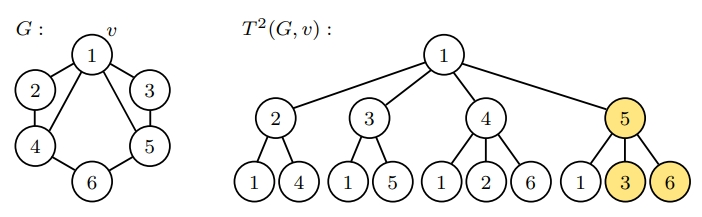
\includegraphics[width=\linewidth]{wwl_unfolding_trees.jpg}
    \caption{The unfolding tree representation of the Weisfeiler-Lehman process is shown. The tree on the right corresponds to the unfolding tree of the node $v$ of the graph shown on the left at a depth of $d=3$.}
    \label{fig:unfolding}
\end{figure}


It is worth noting that, with this unfolding tree representation of a node using the Weisfeiler-Lehman process, the standard Weisfeiler-Lehman kernel would assign a distance of 1 between two unfolding trees if and only if they are isomorphic. To introduce some nuance, the authors proposed to compute the tree edit distance between two trees and using this as a distance measure between two nodes.

The tree edit distance between two trees is the minimal number of operations needed to transform one tree into the other. We consider three different operations: insertion, deletion, and relabeling. While different weights might be given to each operation, the most common approach endows all of them with a uniform weight of 1.

This strategy gives a distance matrix that, according to the authors, reflects more the similarity in between nodes than the previous binary decision. The same process is then applied to this distance matrix as for the standard Wasserstein Weisfeiler-Lehman kernel: the matrix is conditionally negative definite, and therefore the kernel $exp(- \lambda w)$,
where $w$ is the Wasserstein distance computed from this distance matrix, is a positive definite kernel.

Unfortunately, calculating the tree edit distance is a very computationally expensive task.
The state-of-the-art algorithm - Masek and Paterson \cite{masek1980faster}- have worst case runtime of $O(nm/ \log nm)$,
with $m$ and $n$ being the number of nodes of the two unfolding trees,
which is proportional to the number of node and edges in the graph and grows exceptionally with depth.
This is still insufficient for practical applications.
A naïve implementation in Python,
even using multiprocessing and all the previously discussed optimization solutions, shows a runtime superior to a month on our laptops.

To address this issue, we developed a Python module compiled in C++ in the \texttt{treeEditDistance} folder that computes this kernel. Using OpenMP for multithreading, the standard library implementation of trees, a cache system, and state-of-the-art code to compute the Wasserstein distance, we managed to drop the runtime to 24 hours for a depth of $4$.

However, we were not able to achieve this on time to submit our results on Kaggle.
The performance of this kernel can be found in Table \ref{tab:gwwl}.
Surprisingly, the results indicate slightly lower scores than the Wasserstein Weisfeiler-Lehman Kernel,
while this kernel achieves a stunning score of \emph{90.169\%} on Kaggle as shown in Table \ref{tab:summary}.

\begin{table}[h]
    \centering
    \begin{tabular}{l|llll|l}
                & Accuracy & Precision & Recall & F1     & ROCAUC \\
        \hline
        Average & 93.7\%   & 83.3\%    & 39.2\% & 53.5\% & 91.6\% \\
    \end{tabular}
    \caption{\emph{GWWL-edges-depth4} performances.}
    \label{tab:gwwl}
\end{table}

The implementation is split between \texttt{kernel/GWWL.py} for the Python part and \texttt{treeEditDistance/} for the C++ part.

\section{Results and discussions}

\subsection{Summary}
The results of our data project are presented in Table \ref{tab:summary}, which includes the public score computed after submitting on Kaggle.
\emph{Our GWWL method achieved the best overall public score on the leaderboard.}
Unfortunately, this submission was made after the competition deadline
and therefore was not taken into account during the competition.

\begin{table*}[h]
    \centering
    \begin{tabular}{l||cccc|c|c}
        Method (depth) & Accuracy & Precision & Recall & F1              & ROCAUC          & Public Score (Kaggle)  \\
        \hline
        WWL (3)        & 93.9\%   & 87\%      & 39.8\% & 54.5\%          & \textbf{91.8\%} & 89.276\%               \\
        JSWL (6)       & 93.4\%   & 87.5\%    & 33.8\% & 48.6\%          & \textbf{91.8\%} & 88.964\%               \\
        GWWL (4)       & 93.7\%   & 83.3\%    & 39.2\% & 53.3\%          & 91.6\%          & \textbf{90.169\%}  (*) \\
        WL-edges (6)   & 93\%     & 64\%      & 55.1\% & 59.2\%          & 90.3\%          & 85.869\%               \\
        Min-WL (4)     & 93.2\%   & 64.9\%    & 57.8\% & \textbf{61.0\%} & 89.7\%          & 83.194\%               \\
        Minmax-WL (4)  & 93.3\%   & 67.1\%    & 54\%   & 59.8\%          & 89.3\%          & -                      \\
        WL (5)         & 92.6\%   & 61.1\%    & 58\%   & 59.1\%          & 89.3\%          & 81.738\%               \\
        Arithm-WL (4)  & 93.4\%   & 67.7\%    & 54.3\% & 60.3\%          & 88.5\%          & -                      \\
    \end{tabular}
    \caption{Summary of our results. All kernels (except \emph{WL-depth5}) use edges labels during the Weisfeiler-Lehman process.
        (*) This entry was submitted on Kaggle after the challenge deadline, so it is is not taken into account during the competition.
    }
    \label{tab:summary}
\end{table*}

\subsection{On the relative importance of metrics}
First, we would like to draw special attention to the different metrics,
especially the correlation between the F1 score and the AUCROC.
We used all the measures we submitted on Kaggle
(so we could access their online public score)
to compute the correlation matrix shown in Figure \ref{fig:corrmetrics}.
This include the measures presented in Table \ref{tab:summary} and
other submissions.

\begin{figure}[h]
    \centering
    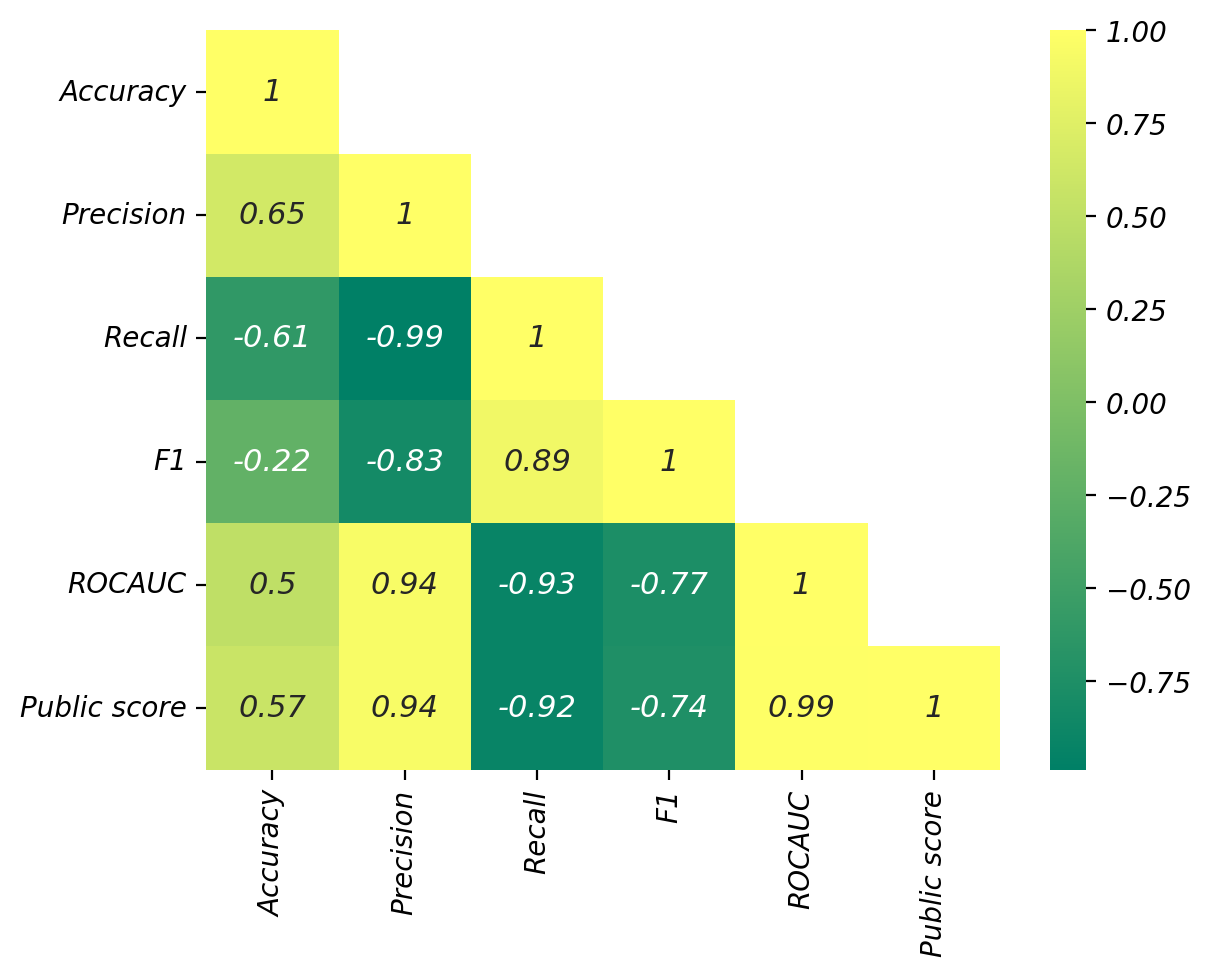
\includegraphics[width=\linewidth]{correlation.png}
    \caption{Correlation matrix between scores, computed with measures taken from \ref{tab:summary} and other submissions.}
    \label{fig:corrmetrics}
\end{figure}

First and most importantly,
our average over cross-validation AUROC is almost perfectly correlated with the public score;
this justifies our approach and gives credit to our methodology.

However, it should be noted that the F1 score is negatively correlated with the AUROC.
We explain this observation by pointing out that the AUROC is more closely correlated with precision rather than recall,
which explains the low correlation with the F1 score.
In our case, since the classes are highly imbalanced,
the balancing property of the F1 opposes the global approach of the AUROC.
Which metric is more relevant depends on the nature of the
problem at hand and can fundamentally change the accepted kernel.
For instance, whether false negatives are acceptable or not, and if a bad recall has an impact on the problem,
are questions that should be answered to ensure that the chosen metric to optimize is relevant.


\subsection{On the correlation between kernels}

Even though all our kernels are based on the same update scheme - the WL process -
we conducted a study to find which kernels were correlated with each other.
Our objective was to determine if two different kernels presenting similar results
were extracting information from the same sources.
The correlation analysis was executed on the predicted outputs for the test set.
Coefficients close to 1 indicate that two kernels are generally predicting
the same activity for the same molecule with a similar level of confidence,
whereas those lower than 1 imply that the two kernels are "more independent",
and hence provide different insights about the molecules.
The correlation matrix is shown in Figure \ref{fig:correlation}.

\begin{figure}[h]
    \centering
    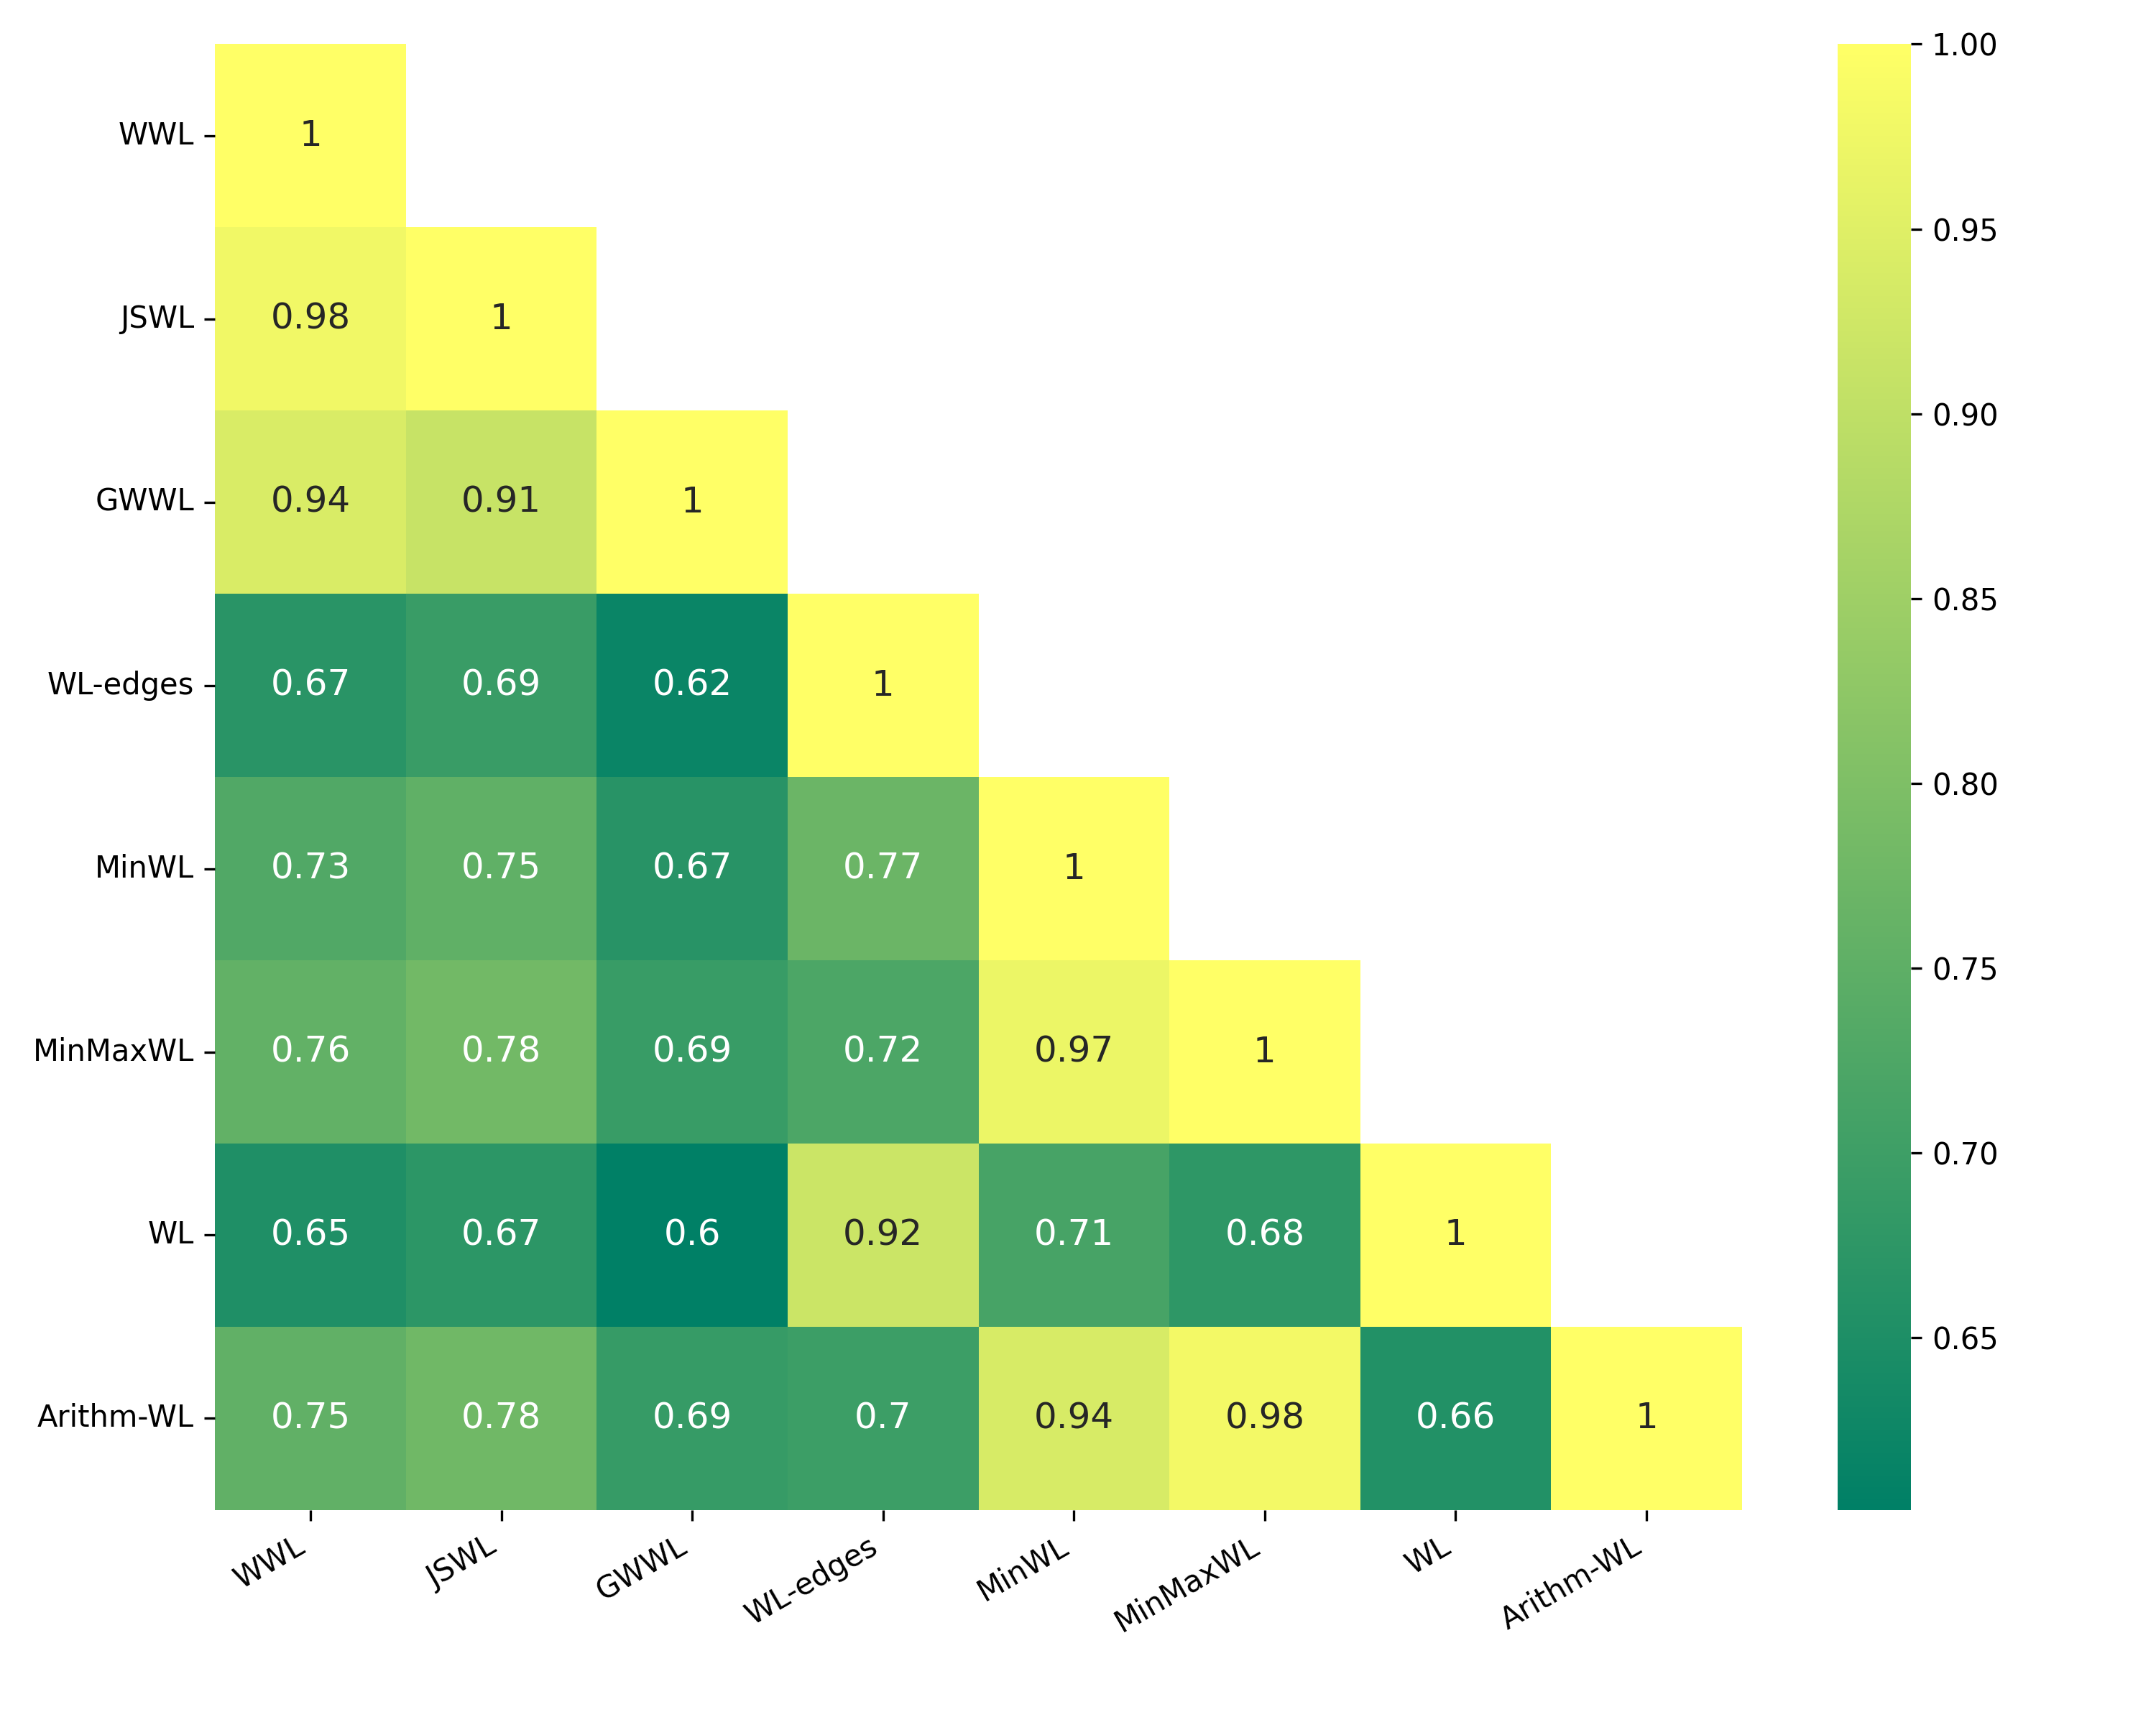
\includegraphics[width=\linewidth]{corr_matrix.png}
    \caption{Correlation matrix between kernels outputs.
        Kernels are in the following order :
        WWL, JSWL, GWWL, WL-edges, MinWL, MinMaxWL, WL and Arithm-WL.
    }
    \label{fig:correlation}
\end{figure}

As expected, since these methods perform quite well,
there is a strong correlation among them
(all coefficients are greater than $0.6$).
Best performing methods are quite similar
as they of course tends to provide the same results.

Therefore, selecting a kernel based on its computational efficiency could be another relevant
criterion to adopt. While these methods exhibit similar performance,
one may take into consideration the day and night difference between the inference time of JSWL and WWL,
for instance.
However, the selection of the criteria depends on the intended usage and resources available to the user.

\section{Conclusion}

In conclusion, we are very pleased with the outcome of this project.
It has not only strengthened our understanding of kernel methods
but has also provided us with a deep insight into state-of-the-art Graph kernels.
We are very proud that our GWWL method would have placed first on the leaderboard if it had been submitted on time.
In addition, we pushed ourselves to attain a decent runtime for all our kernels;
this was a great learning experience, and we were able to gain a wealth of knowledge in computational science.

However, there is still scope for further exploration in the field of Graph Kernels.
We would have liked to try other kernels and ideas if we had more time at our disposal.
Moreover, we did not explore certain concepts such as PCA, which was deliberately put aside due to the time constraint of the challenge.

Overall, this project was deeply interesting and instructive.
Furthermore, the fact that it took place on a concrete domain
with real potential application adds another dimension to our work.
We hope that our research can contribute in any way towards the general study of molecule activity
and serve as a useful reference for future investigations.

\bibliographystyle{plain}
\bibliography{references}

\appendix

\section{Detailed results of our kernels} \label{appendix:allresults}

\begin{table}[!ht]
    \centering
    \begin{tabular}{l||llll|l}
        \textbf{} & \textbf{Accuracy} & \textbf{Precision} & \textbf{Recall} & \textbf{F1} & \textbf{ROCAUC} \\
        \hline \hline
        Fold 1    & 94.5\%            & 65.6\%             & 54.1\%          & 59.3\%      & 87.6\%          \\
        Fold 2    & 92.9\%            & 70.8\%             & 58.3\%          & 64.0\%      & 90.7\%          \\
        Fold 3    & 93.8\%            & 66.7\%             & 54.1\%          & 59.7\%      & 89.6\%          \\
        Fold 4    & 92.6\%            & 70.9\%             & 52.3\%          & 60.2\%      & 87.3\%          \\
        Fold 5    & 94.1\%            & 71.2\%             & 57.8\%          & 63.8\%      & 87.7\%          \\
        Fold 6    & 92.5\%            & 60.8\%             & 49.5\%          & 54.5\%      & 88.3\%          \\
        \hline
        Average   & 93.4\%            & 67.7\%             & 54.3\%          & 60.3\%      & 88.5\%          \\
    \end{tabular}
    \caption{Arithmetic-WL-edges-depth4}
\end{table}

\begin{table}
    \centering
    \begin{tabular}{l||llll|l}
        \textbf{} & \textbf{Accuracy} & \textbf{Precision} & \textbf{Recall} & \textbf{F1} & \textbf{ROCAUC} \\
        \hline \hline
        Fold 1    & 94.4\%            & 75.0\%             & 36.5\%          & 49.1\%      & 92.1\%          \\
        Fold 2    & 92.6\%            & 84.0\%             & 38.9\%          & 53.2\%      & 92.3\%          \\
        Fold 3    & 94.4\%            & 83.7\%             & 42.4\%          & 56.2\%      & 92.6\%          \\
        Fold 4    & 92.9\%            & 87.5\%             & 39.3\%          & 54.2\%      & 90.6\%          \\
        Fold 5    & 94.3\%            & 90.2\%             & 41.1\%          & 56.5\%      & 90.6\%          \\
        Fold 6    & 93.4\%            & 79.1\%             & 37.4\%          & 50.7\%      & 91.2\%          \\
        \hline
        Average   & 93.7\%            & 83.3\%             & 39.2\%          & 53.3\%      & 91.6\%          \\
    \end{tabular}
    \caption{GWWL-edges-depth4}
\end{table}

\begin{table}
    \centering
    \begin{tabular}{l||llll|l}
        \textbf{} & \textbf{Accuracy} & \textbf{Precision} & \textbf{Recall} & \textbf{F1} & \textbf{ROCAUC} \\
        \hline \hline
        Fold 1    & 94.7\%            & 83.9\%             & 35.1\%          & 49.5\%      & 91.0\%          \\
        Fold 2    & 92.1\%            & 82.2\%             & 34.3\%          & 48.4\%      & 93.0\%          \\
        Fold 3    & 94.4\%            & 89.2\%             & 38.8\%          & 54.1\%      & 92.9\%          \\
        Fold 4    & 92.4\%            & 87.8\%             & 33.6\%          & 48.6\%      & 91.1\%          \\
        Fold 5    & 94.1\%            & 97.0\%             & 35.6\%          & 52.0\%      & 91.1\%          \\
        Fold 6    & 92.8\%            & 85.2\%             & 25.3\%          & 39.0\%      & 91.8\%          \\
        \hline
        Average   & 93.4\%            & 87.5\%             & 33.8\%          & 48.6\%      & 91.8\%          \\
    \end{tabular}
    \caption{JSWL-edges-depth6}
\end{table}

\begin{table}
    \centering
    \begin{tabular}{l||llll|l}
        \textbf{} & \textbf{Accuracy} & \textbf{Precision} & \textbf{Recall} & \textbf{F1} & \textbf{ROCAUC} \\
        \hline \hline
        Fold 1    & 94.8\%            & 66.2\%             & 60.8\%          & 63.4\%      & 89.2\%          \\
        Fold 2    & 92.6\%            & 67.7\%             & 60.2\%          & 63.7\%      & 91.1\%          \\
        Fold 3    & 93.7\%            & 65.7\%             & 54.1\%          & 59.4\%      & 90.6\%          \\
        Fold 4    & 92.2\%            & 67.5\%             & 52.3\%          & 58.9\%      & 87.5\%          \\
        Fold 5    & 92.8\%            & 59.2\%             & 64.4\%          & 61.7\%      & 89.6\%          \\
        Fold 6    & 93.0\%            & 63.3\%             & 54.9\%          & 58.8\%      & 90.0\%          \\
        \hline
        Average   & 93.2\%            & 64.9\%             & 57.8\%          & 61.0\%      & 89.7\%          \\
    \end{tabular}
    \caption{Min-WL-edges-depth4}
\end{table}


\begin{table}
    \centering
    \begin{tabular}{l||llll|l}
        \textbf{} & \textbf{Accuracy} & \textbf{Precision} & \textbf{Recall} & \textbf{F1} & \textbf{ROCAUC} \\
        \hline \hline
        Fold 1    & 94.7\%            & 66.7\%             & 56.8\%          & 61.3\%      & 88.8\%          \\
        Fold 2    & 92.4\%            & 67.8\%             & 56.5\%          & 61.6\%      & 90.5\%          \\
        Fold 3    & 93.8\%            & 66.7\%             & 54.1\%          & 59.7\%      & 90.0\%          \\
        Fold 4    & 92.3\%            & 69.7\%             & 49.5\%          & 57.9\%      & 88.3\%          \\
        Fold 5    & 94.2\%            & 72.9\%             & 56.7\%          & 63.7\%      & 88.7\%          \\
        Fold 6    & 92.3\%            & 59.0\%             & 50.5\%          & 54.4\%      & 89.3\%          \\
        \hline
        Average   & 93.3\%            & 67.1\%             & 54.0\%          & 59.8\%      & 89.3\%          \\
    \end{tabular}
    \caption{MinMax-WL-edges-depth4}
\end{table}



\begin{table}
    \centering
    \begin{tabular}{l||llll|l}
        \textbf{} & \textbf{Accuracy} & \textbf{Precision} & \textbf{Recall} & \textbf{F1} & \textbf{ROCAUC} \\
        \hline \hline
        Fold 1    & 93.8\%            & 58.8\%             & 54.1\%          & 56.3\%      & 88.3\%          \\
        Fold 2    & 89.9\%            & 52.6\%             & 66.7\%          & 58.8\%      & 89.7\%          \\
        Fold 3    & 93.5\%            & 62.5\%             & 58.8\%          & 60.6\%      & 90.5\%          \\
        Fold 4    & 92.1\%            & 67.1\%             & 51.4\%          & 58.2\%      & 87.3\%          \\
        Fold 5    & 92.9\%            & 62.3\%             & 53.3\%          & 57.5\%      & 88.3\%          \\
        Fold 6    & 93.3\%            & 63.0\%             & 63.7\%          & 63.4\%      & 91.3\%          \\
        \hline
        Average   & 92.6\%            & 61.1\%             & 58.0\%          & 59.1\%      & 89.3\%          \\
    \end{tabular}
    \caption{WL-depth5}
\end{table}


\begin{table}
    \centering
    \begin{tabular}{l||llll|l}
        \textbf{} & \textbf{Accuracy} & \textbf{Precision} & \textbf{Recall} & \textbf{F1} & \textbf{ROCAUC} \\
        \hline \hline
        Fold 1    & 94.6\%            & 64.7\%             & 59.5\%          & 62.0\%      & 90.2\%          \\
        Fold 2    & 91.4\%            & 62.0\%             & 52.8\%          & 57.0\%      & 89.9\%          \\
        Fold 3    & 93.7\%            & 64.1\%             & 58.8\%          & 61.3\%      & 92.9\%          \\
        Fold 4    & 91.1\%            & 61.3\%             & 45.8\%          & 52.4\%      & 87.0\%          \\
        Fold 5    & 93.5\%            & 67.1\%             & 54.4\%          & 60.1\%      & 90.9\%          \\
        Fold 6    & 93.4\%            & 65.1\%             & 59.3\%          & 62.1\%      & 91.2\%          \\
        \hline
        Average   & 93.0\%            & 64.0\%             & 55.1\%          & 59.2\%      & 90.3\%          \\
    \end{tabular}
    \caption{WL-edges-depth6}
\end{table}


\begin{table}
    \centering
    \begin{tabular}{l||llll|l}
        \textbf{} & \textbf{Accuracy} & \textbf{Precision} & \textbf{Recall} & \textbf{F1} & \textbf{ROCAUC} \\
        \hline \hline
        Fold 1    & 95.0\%            & 83.3\%             & 40.5\%          & 54.5\%      & 91.7\%          \\
        Fold 2    & 92.4\%            & 82.0\%             & 38.0\%          & 51.9\%      & 92.3\%          \\
        Fold 3    & 94.7\%            & 88.1\%             & 43.5\%          & 58.3\%      & 92.5\%          \\
        Fold 4    & 93.0\%            & 87.8\%             & 40.2\%          & 55.1\%      & 91.5\%          \\
        Fold 5    & 94.6\%            & 95.0\%             & 42.2\%          & 58.5\%      & 90.3\%          \\
        Fold 6    & 93.5\%            & 86.1\%             & 34.1\%          & 48.8\%      & 92.4\%          \\
        \hline
        Average   & 93.9\%            & 87.0\%             & 39.8\%          & 54.5\%      & 91.8\%          \\
    \end{tabular}
    \caption{WWL-edges-depth3}
\end{table}
\end{document}
